Viele Probleme der KI lassen sich auf eine systematische Suche in einem Wurzelbaum reduzieren. \\
Problem: Riesige Anzahl von Knoten in typischen Suchbäumen. 
\cparagraph{Beispiel} Schachspiel, ca. $30$ Möglichkeiten pro Halbzug (Zug einer Farbe). Bei $50$ Halbzügen enthält der Suchbaum:
$$\sum_{d=0}^{50} 30^d = \frac{30^{51}-1}{30-1} \approx 7,4 \cdot 10^{73}\unit{Knoten}$$
Bei $10\, 000$ Computern, die $10^9 \unit{Knoten/s}$ erzeugen und durchsuchen können, würde das durchsuchen so lange dauern:
$$ \frac{7,4 \cdot 10^{73}}{10\,000 \cdot 10^9}\unit{s}=2,3 \cdot 10^{53} \unit{Jahre}$$

\section{Uninformierte Suche}
Bereits bekannt: Breiten- und Tiefensuche. Zur Implementierung in Prolog benötigen wir:
\begin{itemize}
\item \lstinline`findall(X, P, L)`: Sucht alle \lstinline`X`, für die \lstinline`P` wahr ist und erzeugt daras die Liste \lstinline`L`.
\item \lstinline`not(P)`: Ist wahr genau dann, wenn Prolog \lstinline`P` nicht beweisen kann („Negation by failure“).
\end{itemize}
\subsection{Breitensuche}
\begin{lstlisting}[language=Prolog]
% Adjazenzrelation des ungerichteten Graphen (nicht effizient)
adj(X,Y) :- adj0(X,Y); adj0(Y,X).
adj0(X,Y) :- member((X,Y), [(1,2), (2,4), (2,5), (3,4), (3,6), (4,5)]).

goal(6).

% Breitensuche
bfs([H|T], Discovered) :-
	goal(H);
	findall(Node, (adj(H, Node), not(member(Node, Discovered))), NewNeighbors),
	append(T, NewNeighbors, Queue),
	append(Discovered, NewNeighbors, Dc),
	write('Queue: '), writeln(Queue), % zur Illustration
	bfs(Queue, Dc).
\end{lstlisting}

Starten der Breitensuche beim Knoten $1$:
\begin{lstlisting}[language=Prolog]
?- bfs([1], [1]).
Queue: [2]
Queue: [4,5]
Queue: [5,3]
Queue: [3]
Queue: [6]
true .
\end{lstlisting}
\subsection{Problem der Breiten- und Tiefensuche} 
Wenn alle bereits besuchten Knoten gespeichert werden: Exponentielle Laufzeit und exponentieller Speicherplatzbedarf (für die Discoverd-Liste) in der Tiefe des Baumes.
\subsection{Tiefensuche}
Einfach: aus \lstinline`append(T, NewNeighbors, Queue)` wird \lstinline`append(NewNeighbors, T, Queue`.\\
Ohne expliziten Stack, Knoten auf aktuellen Pfad werden gespeichert (nicht alle Knoten wie bei Discovered $\to$ vermeidet exponentiellen Speicherplatzbedarf -- funktioniert, da der zu durchsuchende Graph in der Regel ein Baum ist [Knoten könnten nur durch Schleifen doppelt besucht werden]):
\begin{lstlisting}[language=Prolog]
% Adjazenzrelation des ungerichteten Graphen (nicht effizient)
adj(X,Y) :- adj0(X,Y); adj0(Y,X).
adj0(X,Y) :- member((X,Y), [(1,2), (2,4), (2,5), (3,4), (3,6), (4,5)]).

goal(6).

dfs3(Node, Path) :-
	goal(Node);
	adj(Node, NewNeighbor), not(member(NewNeighbor,Path)),
	write('Knoten: '), writeln(NewNeighbor), % zur Illustration
	dfs3(NewNeighbor, [NewNeighbor|Path]).

% Wie dfs3, gefundener ReturnPath wird zurückgegeben
dfs4(Node, Path, ReturnPath) :-
	goal(Node), reverse(Path, ReturnPath);
	adj(Node,NewNeighbor), not(member(NewNeighbor,Path)),
	dfs4(NewNeighbor, [NewNeighbor|Path], ReturnPath).
\end{lstlisting}

\subsection{Vorteile/Nachteile Breiten- und Tiefensuche}
\lecdate{22.05.2017}
\subsubsection*{Breitensuche}
\begin{itemize}
\item[$+$] Liefert kürzesten Pfad, funktioniert auch für unendliche Graphen.
\item[$-$] Alle Knoten werden gespeichert.
\end{itemize}

\subsubsection*{Tiefensuche}
\begin{itemize}
\item[$+$] Nur die Knoten auf dem aktuellen Pfad werden gespeichert.
\item[$-$] Liefert nicht immer den kürzesten Pfad und funktioniert nicht für unendliche Graphen.\\
Beispiel:
\begin{center}
% Credits: 3evilcookie
\begin{tikzpicture}
\draw  (0,0) node (v1) {} rectangle (8,3);
\draw  [pattern = north west lines,pattern color=gray](v1) rectangle (1,1);
\draw  [pattern = north west lines,pattern color=gray](2,1) rectangle (3,0);
\draw  [pattern = north west lines,pattern color=gray](4,1) rectangle (5,0);
\draw  [pattern = north west lines,pattern color=gray](6,1) rectangle (7,0);
\draw  [pattern = north west lines,pattern color=gray](1,2) node (v3) {} rectangle (2,1);
\draw  [pattern = north west lines,pattern color=gray](3,2) rectangle (4,1);
\draw  [pattern = north west lines,pattern color=gray](5,2) rectangle (6,1);
\draw  [pattern = north west lines,pattern color=gray](7,2) rectangle (8,1);
\node (v2) at (0.5,0.5) {O};
\draw [-latex,dashed,red](v2) -- (7.5,0.5) -- (7.5,1.5) -- (0.5,1.5) -- (0.5,2.5) -- (7.5,2.5);
\draw  [pattern = north west lines,pattern color=gray](v3) rectangle (0,3);
\draw  [pattern = north west lines,pattern color=gray](2,2) rectangle (3,3);
\draw  [pattern = north west lines,pattern color=gray](4,2) rectangle (5,3);
\draw  [pattern = north west lines,pattern color=gray](6,2) rectangle (7,3);
\end{tikzpicture}
\end{center}
\end{itemize}

%Bei der Tiefensuche kann es vorkommen, dass ein ungünstiger Pfad zum Ziel gefunden wird. Das Problem kann man mit der iterativen Tiefensuche lösen:

\subsection{Iterative Tiefensuche}
Wir verwenden eine Tiefensuche mit einer Tiefenschranke, die sukzessive erhöht wird, bis das Ziel gefunden ist.
\begin{center}
% Credits: 3evilcookie
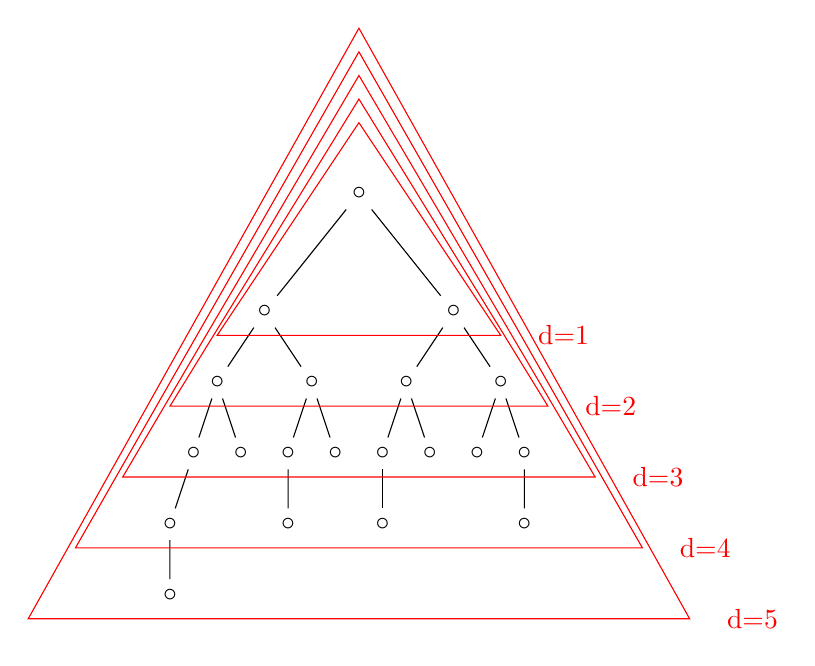
\begin{tikzpicture}[scale=.6]
\draw  (0,4) node (v1) {$\circ$};
\draw  (-2,1.5) node (v2) {$\circ$};
\draw  (2,1.5) node (v7) {$\circ$};
\draw  (-3,0) node (v3) {$\circ$};
\draw  (-1,0) node (v4) {$\circ$};
\draw  (1,0) node (v8) {$\circ$};
\draw  (3,0) node (v11) {$\circ$};
\draw  (-3.5,-1.5) node (v16) {$\circ$};
\draw  (-2.5,-1.5) node (v22) {$\circ$};
\draw  (-1.5,-1.5) node (v5) {$\circ$};
\draw  (-0.5,-1.5) node (v6) {$\circ$};
\draw  (3.5,-1.5) node (v13) {$\circ$};
\draw  (2.5,-1.5) node (v12) {$\circ$};
\draw  (1.5,-1.5) node (v10) {$\circ$};
\draw  (0.5,-1.5) node (v9) {$\circ$};
\draw (v1) -- (v2) -- (v3) -- (v16) (v2) -- (v4);
\draw (v4) -- (v5) (v3) -- (v22) (v4) -- (v6) (v1) -- (v7) -- (v8) -- (v9) (v8) -- (v10) (v7) -- (v11) -- (v12) (v11) -- (v13);
\draw  (-4,-3) node (v17) {$\circ$};
\draw  (-4,-4.5) node (v18) {$\circ$};
\draw  (-1.5,-3) node (v19) {$\circ$};
\draw  (0.5,-3) node (v20) {$\circ$};
\draw  (3.5,-3) node (v21) {$\circ$};
\draw [red](-3,1) -- (3,1)node[right = 1em]{d=1} -- (0,5.5) -- cycle;
\draw [red](-4,-0.5) -- (4,-0.5)node[right = 1em]{d=2} -- (0,6) -- cycle;
\draw (v16) -- (v17) -- (v18);
\draw (v5) -- (v19);
\draw (v9) -- (v20);
\draw (v13) -- (v21);
\draw [red] (-5,-2) -- (5,-2)node[right = 1em]{d=3} --(0,6.5) -- cycle;
\draw [red](-6,-3.5) -- (6,-3.5)node[right = 1em]{d=4} -- (0,7) -- cycle;
\draw [red](-7,-5) -- (7,-5)node[right = 1em]{d=5} -- (0,7.5) -- cycle;
\end{tikzpicture}
\end{center}
Die iterative Tiefensuche besitzt damit alle Vorteile.\\
Zur Rechenzeit: Diese ist länger als bei der Breitensuche, da alle vorherigen Kanten nochmal besucht werden.\\
In einem Suchbaum mit Verzweigungsfaktor $>1$ sind fast alle Knoten Blätter. Daher fällt auch die meiste Rechenzeit für das Durchsuchen der Blätter an. Durch eine genaue Rechnung lässt sich zeigen, dass die Laufzeit der iterativen Tiefensuche nur um einen kleinen Faktor höher ist als die der Tiefensuche.

\begin{lstlisting}[language=Prolog]
% Node: aktueller Knoten
% Goal: Zielknoten
% Path: Liste der Knoten auf dem Pfad bis Node
% ReturnPath: Rückgabe, wenn ein Pfad zum Ziel gefunden wurde
dlDfs(Node, Goal, Path, DepthLimit, ReturnPath) :-
	Node = Goal, reverse(Path, ReturnPath);
	DepthLimit > 0,
	adj(Node,NewNeighbor), not(member(NewNeighbor,Path)),
	dlDfs(NewNeighbor, Goal, [NewNeighbor|Path], DepthLimit-1, ReturnPath).

idDfsLoop(Start, Goal, D, ReturnPath) :-
	dlDfs(Start, Goal, [Start], D, ReturnPath);
	% Wenn die Tiefensuche mit Schranke D nicht erfolgreich war, wird mit Schranke D+1 weitergesucht.
	idDfsLoop(Start, Goal, D+1, ReturnPath).

idDfs(Start, Goal, ReturnPath) :- idDfsLoop(Start, Goal, 1, ReturnPath).

\end{lstlisting}

\subsubsection{Anwendung: Planungsproblem}
Affe-Banane-Problem\\
Situation: Raum mit
\begin{itemize}
\item Affe an der Tür
\item Banane an der Decke in der Mitte des Raumes
\item Stuhl am Fenster
\end{itemize}
Ziel: Affe soll die Banane greifen.\\
Regeln: Affe kann laufen, den Stuhl verschieben, auf den Stuhl steigen, die Banane greifen, wenn er unter der Banane auf dem Stuhl steht.\\
Zugehöriger Graph, der das Suchproblem darstellt: Knoten sind Situationen, Kanten entsprechen den anwendbaren Regeln.
\begin{center}
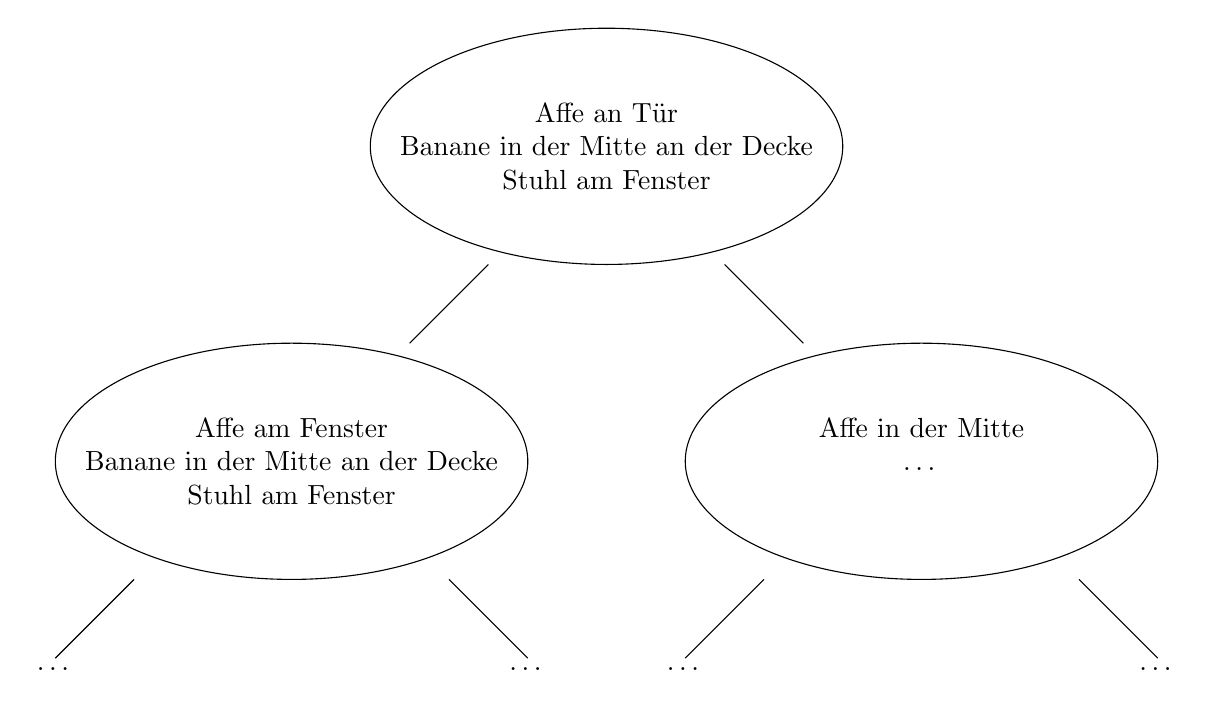
\begin{tikzpicture}[align= center]
\draw (0,0) node{Affe an Tür\\
Banane in der Mitte an der Decke\\
Stuhl am Fenster} ellipse (3 and 1.5);
\draw (-4,-4) node{Affe am Fenster\\
Banane in der Mitte an der Decke\\
Stuhl am Fenster} ellipse (3 and 1.5);
\draw (4,-4) node{Affe in der Mitte\\
…\\
~} ellipse (3 and 1.5);
\draw (-2.5,-2.5) -- (-1.5,-1.5);
\draw (2.5,-2.5) -- (1.5,-1.5);
\draw (-7,-6.5) node[below]{…} -- (-6,-5.5);
\draw (-1,-6.5) node[below]{…} -- (-2,-5.5);
\draw (1,-6.5) node[below]{…} -- (2,-5.5);
\draw (7,-6.5) node[below]{…} -- (6,-5.5);
\end{tikzpicture}
\end{center}

\begin{lstlisting}[language=Prolog]
:- [idDfs].	% entspricht include

ort(X) :- member(X, [tuer, mitte, fenster]).
% Bedeutung der Listen: [Affe, Banane, Stuhl, Affe auf Stuhl]
adj0([A1,B,S,f], [A2,B,S,f]) :- ort(A1), ort(A2).		% laufen
adj0([A1,B,A1,f], [A2,B,A2,f]) :- ort(A1), ort(A2).		% Stuhl schieben
adj0([A,B,A,f], [A,B,A,t]).		% auf Stuhl steigen
goal([A,A,_,t]).		% Banane greifen

adj(X,Y) :- adj0(X,Y); adj0(Y,X).

solution(Path) :- Start = [tuer, mitte, fenster, f], goal(Goal), idDfs(Start,Goal,Path).
\end{lstlisting}

\section{Informierte Suche (heuristische Suche)}
\lecdate{29.05.2017}
Ziel: Information über das Suchproblem nutzen, um gute Pfade zuerst zu verfolgen. Dabei wird eine Bewertungsfunktion für die Knoten verwendet.\\
Die heuristische Suche verwendet eine heuristische Bewertungsfunktion $f: V\to \RR_0^+$. Für den Zielknoten $v$ gilt $f(v)=0$. Die Knoten mit der niedrigsten Bewertung werden zuerst verfolgt.
\subsection{Gierige Suche} Verwendet in jedem Schritt den Knoten, der dem Ziel am nächsten liegt.

\cparagraph{Beispiel} Suche nach kürzestem Weg zu einem Ort $f(v)=\text{Luftlinienentfernung zum Ziel}$
\begin{center}
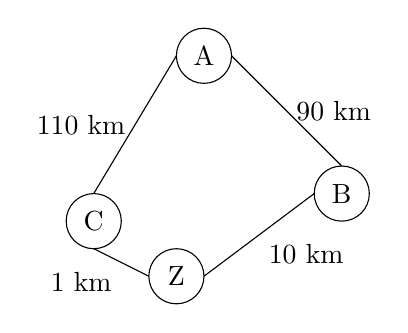
\begin{tikzpicture}[scale=.7]
\draw  (-2.5,2.5) node{A} ellipse (0.5 and 0.5);
\draw  (-4.5,-0.5) node{C} ellipse (0.5 and 0.5);
\draw  (0,0) node{B} ellipse (0.5 and 0.5);
\draw  (-3,-1.5) node{Z} ellipse (0.5 and 0.5);
\draw (-3,2.5) -- node[left]{110 km} (-4.5,0);
\draw (-4.5,-1) -- node[below left]{1 km} (-3.5,-1.5);
\draw (-2,2.5) -- node[right]{90 km} (0,0.5);
\draw (-2.5,-1.5) -- node[below right]{10 km} (-0.5,0);
\end{tikzpicture}
\end{center}
Die gierige Suche verfolgt den Weg A--C--Z (111 km). Dabei ist A--B--Z (100 km) kürzer.

\subsection{A*-Suche}
Die gierige Suche berücksichtigt nicht die Kosten, die bis zum Knoten $v$ bereits entstanden sind. Wir führen daher eine Funktion $g$ ein, die die Kosten vom Startknoten bis $v$ angibt (also der bereits zurückgelegte Weg) und eine Funktion $h$, die die (verbleibenden) Kosten bis zum Ziel schätzt.\\
Daher definieren wir die heuristische Bewertungsfunktion $f$ durch:
$$f(v)=g(v)+h(v)$$
Der A*-Algorithmus verwendet eine Bewertungsfunktion $f$, die die Summe der Kosten bis $v$ und die geschätzten Kosten bis zum Ziel sind. Dabei muss $h$ zulässig sein.
\cparagraph{Definition} Eine heuristische Kostenschätzfunktion $h$ heißt \emph{zulässig}, wenn $h$ die Kosten bis zum Ziel nie überschätzt.
\cparagraph{Beispiel}
\begin{itemize}
\item Die Luftlinienentfernung bis zum Ziel ist eine zulässige Kostenschätzfunktion.
\item $0$ (aber nicht nützlich, $\to$ gierige Suche).
\end{itemize}
\bigskip

\subsubsection{Implementierung durch Liste (ineffizient)}
Für jeden aktuellen Konten $u$ werden die noch unbesuchten Nachbarn $v$ bestimmt und diese entsprechend ihrer $f$-Werte sortiert in eine Liste der nach zu besuchenden Knoten eingefügt. Wenn die Liste dabei in jedem Schritt neu sortiert wird, entsteht jeweils ein Aufwand von $O(n \log n)$.
\subsubsection{Implementierung durch Min-Heap}
Eine effiziente Implementierung verwendet einen \emph{Min-Heap}.\\
Ein Min-Heap ist ein Binärbaum, in dem jeder Knoten, der kein Blatt ist, einen kleineren oder maximal gleichen Wert besitzt als alle Nachfolger.
\cparagraph{Beispiel}
\begin{center}
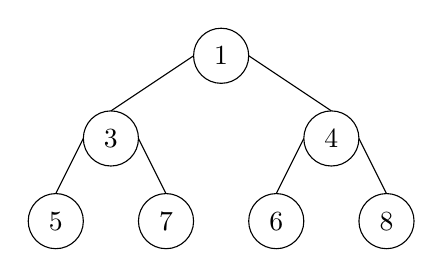
\begin{tikzpicture}[scale=.7]
\draw  (-1,3.5) node{1} ellipse (0.5 and 0.5);
\draw  (-3,2) node{3} ellipse (0.5 and 0.5);
\draw  (1,2) node{4} ellipse (0.5 and 0.5);
\draw  (-4,0.5) node{5} ellipse (0.5 and 0.5);
\draw  (-2,0.5) node{7} ellipse (0.5 and 0.5);
\draw  (0,0.5) node{6} ellipse (0.5 and 0.5);
\draw  (2,0.5) node{8} ellipse (0.5 and 0.5);
\draw (-1.5,3.5) -- (-3,2.5);
\draw (-3.5,2) -- (-4,1);
\draw (-2.5,2) -- (-2,1);
\draw (-0.5,3.5) -- (1,2.5);
\draw (0.5,2) -- (0,1);
\draw (1.5,2) -- (2,1);
\end{tikzpicture}
\end{center}
Alle wichtigen Heap-Operationen (\lstinline`readMin, add`) können in der Zeit $O(\log n)$ ausgeführt werden.\\
Eine effiziente A*-Suche verwendet einen Min-Heap, um die Knoten entsprechend ihrer $f$-werte zu verwalten. Dadurch fällt in jedem Schritt nur noch ein zusätzlicher Aufwand von $O(\log n)$ an.\bigskip\\
Die A*-Suche ist optimal, d.h., sie findet einen kürzesten Weg.

\subsubsection{Vor-/Nachteile}
\begin{itemize}
\item[$+$] Bei guter Heuristik wird das Ziel oft wesentlich schneller gefunden als mit einer uninformierten Suche.
\item[$-$] Hoher Speicherbedarf, weil im worst-Case alle Knoten gespeichert werden müssen.
\item[$-$] (wie bei Breitensuche:) es ist nicht einfach möglich den gefundenen Pfad zurückzugeben. 
\end{itemize}

\begin{lstlisting}[language=Prolog]
% Heuristische Bewertungsfunktion
% [H|T]: Pfad zum aktuellen Knoten H
f([H|T],Y) :- g([H|T],Y1), h(H,Y2), Y is Y1+Y2.
g(L,Y) :- length(L,Y1), Y is Y1-1.
h(X,Y) :- Y is 0. % Ändern! Hier muß eine Kostenschätzfunktion angegeben werden.

% A*-Suche
% [H|T]: Sortierte Liste der noch zu untersuchenden Knoten
% Closed: Liste der Knoten, die bereits untersucht wurden
% Die Knoten müssen hier Pfade zum aktuellen, eigentlichen Knoten sein, damit f dessen Bewertung berechnen kann.
hs([H|T], Closed) :-
	goal(H);
	Cl = [H|Closed],
	findall(Node, (adj(H, Node), not(member(Node, Cl))), NewNeighbors),
	append(T, NewNeighbors, Queue),
	fsort(Queue, SortedQ),
	hs(SortedQ, Cl).
	
% Sortieren der Liste gemäß der Werte von f
fsort(List, Sorted) :- 
        map_list_to_pairs(f, List, Pairs), 
        keysort(Pairs, SortedPairs), 
        pairs_values(SortedPairs, Sorted). 
\end{lstlisting}

\subsection{IDA*-Suche}
\lecdate{12.06.2017}
Die IDA*-Suche kombiniert die Vorteile der A*-Suche mit denen der iterativen Tiefensuche. Anstelle der Tiefenschranke der iterativen Tiefensuche verwenden wir eine Schranke für die Werte der Bewertungsfunktion. Der Speicherbedarf der IDA*-Suche entspricht dem der Tiefensuche.

\begin{lstlisting}[language=Prolog]
% f: Heuristische Bewertungsfunktion
% h: Heuristische Kostenschätzfunktion
% [Head|Tail]: Aktueller Pfad, Head: aktueller Knoten 
f([Head|Tail], F) :- 
	length(Tail, G),
	h(Head, H),
	F is G+H. 

% Node: aktueller Knoten
% Goal: Zielknoten
% Path: Liste der Knoten auf dem Pfad bis Node
% ReturnPath: Rückgabe, wenn ein Pfad zum Ziel gefunden wurde
% adj: Adjazenz eines Knotens
flDfs(Node, Goal, Path, FLimit, ReturnPath) :-
	Node == Goal, reverse(Path, ReturnPath);
	adj(Node,NewNeighbor), not(member(NewNeighbor,Path)),
	f([NewNeighbor|Path], F), F =< FLimit,
	flDfs(NewNeighbor, Goal, [NewNeighbor|Path], FLimit, ReturnPath).

idasLoop(Start, Goal, FLimit, ReturnPath) :-
	flDfs(Start, Goal, [Start], FLimit, ReturnPath);
	% Schranke für f wird um kleinstmögliche Schrittweite erhöht (einfach zu programmieren). Sie wird also erhöht, wenn Ziel noch nicht gefunden wurde, um den Radius zu erhöhen.
	idasLoop(Start, Goal, FLimit+1, ReturnPath).

idas(Start, Goal, ReturnPath) :-
	% Da f zulässig ist, sind die Kosten bis zum Ziel mindestens FL
	f([Start], FLimit),
	idasLoop(Start, Goal, FLimit, ReturnPath).
\end{lstlisting}

\paragraph{Anwendung} 8-Punkte\\
Ziel: Plättchen in folgende Stellung zu bringen:
\begin{center}
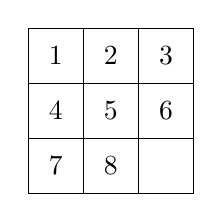
\begin{tikzpicture}[scale=.7]
\draw  (0,0) rectangle node{1} (1,-1);
\draw  (1,0) rectangle node{2} (2,-1);
\draw  (2,0) rectangle node{3} (3,-1);
\draw  (0,-1) rectangle node{4} (1,-2);
\draw  (1,-1) rectangle node{5} (2,-2);
\draw  (2,-1) rectangle node{6} (3,-2);
\draw  (0,-2) rectangle node{7} (1,-3);
\draw  (1,-2) rectangle node{8} (2,-3);
\draw  (2,-2) rectangle node{} (3,-3);
\end{tikzpicture}
\end{center}
Darstellung als Graph:
\begin{itemize}
\item Knoten: Brettstellungen
\item Kanten: Übergänge, die durch das Verschieben eines Plättchen möglich sind.
\end{itemize}
Beispiel:
\begin{center}
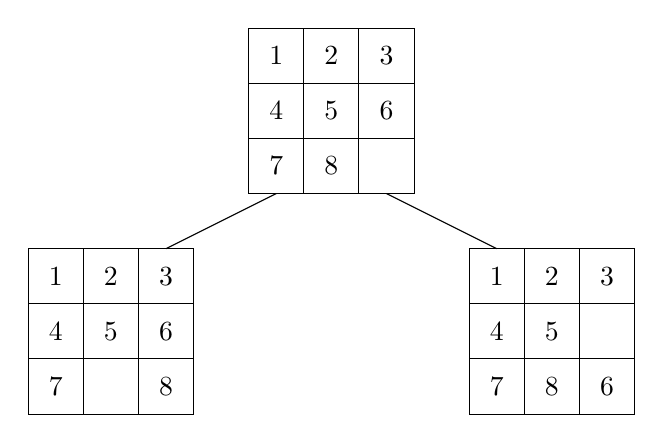
\begin{tikzpicture}[scale=.7]
\draw  (0,0) rectangle node{1} (1,-1);
\draw  (1,0) rectangle node{2} (2,-1);
\draw  (2,0) rectangle node{3} (3,-1);
\draw  (0,-1) rectangle node{4} (1,-2);
\draw  (1,-1) rectangle node{5} (2,-2);
\draw  (2,-1) rectangle node{6} (3,-2);
\draw  (0,-2) rectangle node{7} (1,-3);
\draw  (1,-2) rectangle node{8} (2,-3);
\draw  (2,-2) rectangle node{} (3,-3);

\draw  (4,-4) rectangle node{1} (5,-5);
\draw  (5,-4) rectangle node{2} (6,-5);
\draw  (6,-4) rectangle node{3} (7,-5);
\draw  (4,-5) rectangle node{4} (5,-6);
\draw  (5,-5) rectangle node{5} (6,-6);
\draw  (6,-5) rectangle node{} (7,-6);
\draw  (4,-6) rectangle node{7} (5,-7);
\draw  (5,-6) rectangle node{8} (6,-7);
\draw  (6,-6) rectangle node{6} (7,-7);

\draw  (-4,-4) rectangle node{1} (-3,-5);
\draw  (-3,-4) rectangle node{2} (-2,-5);
\draw  (-2,-4) rectangle node {3} (-1,-5);
\draw  (-4,-5) rectangle node{4} (-3,-6);
\draw  (-3,-5) rectangle node{5} (-2,-6);
\draw  (-2,-5) rectangle node{6} (-1,-6);
\draw  (-4,-6) rectangle node{7} (-3,-7);
\draw  (-3,-6) rectangle node{} (-2,-7);
\draw  (-2,-6) rectangle node{8} (-1,-7);

\draw (0.5,-3) -- (-1.5,-4);
\draw (2.5,-3) -- (4.5,-4);
\end{tikzpicture}
\end{center}
Geeignete heuristische Kostenschätzfunktionen $h$:
\begin{enumerate}
\item Hamming-Distanz bis zum Ziel:\\
Die Hamming-Distanz zweier Plättchen ist die Anzahl der Plättchen, in denen sich die Stellungen unterscheiden.\\
Beispiel:
\begin{center}
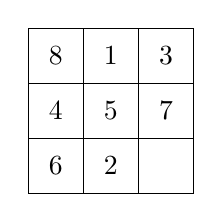
\begin{tikzpicture}[scale=0.7]
\draw  (0,0) rectangle node{8} (1,-1);
\draw  (1,0) rectangle node{1} (2,-1);
\draw  (2,0) rectangle node{3} (3,-1);
\draw  (0,-1) rectangle node{4} (1,-2);
\draw  (1,-1) rectangle node{5} (2,-2);
\draw  (2,-1) rectangle node{7} (3,-2);
\draw  (0,-2) rectangle node{6} (1,-3);
\draw  (1,-2) rectangle node{2} (2,-3);
\draw  (2,-2) rectangle node{} (3,-3);
\end{tikzpicture}
\end{center}
$$h=1+1+0+0+0+1+1+1=5$$
Diese Heuristik ist zulässig, weil mindestens so viele Verschiebungen von Plättchen nötig sind, wie Plättchen falsch stehen.
\item Manhatten- oder Cityblock-Distanz:\\
Anzahl der Verschiebungen, die nötig sind, um ein Plättchen auf direktem Weg zur Zielposition zu schieben, summiert über alle Plättchen.\\
Beispiel:
\begin{center}
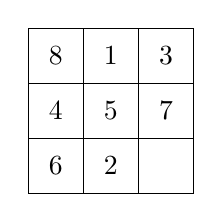
\begin{tikzpicture}[scale=0.7]
\draw  (0,0) rectangle node{8} (1,-1);
\draw  (1,0) rectangle node{1} (2,-1);
\draw  (2,0) rectangle node{3} (3,-1);
\draw  (0,-1) rectangle node{4} (1,-2);
\draw  (1,-1) rectangle node{5} (2,-2);
\draw  (2,-1) rectangle node{7} (3,-2);
\draw  (0,-2) rectangle node{6} (1,-3);
\draw  (1,-2) rectangle node{2} (2,-3);
\draw  (2,-2) rectangle node{} (3,-3);
\end{tikzpicture}
\end{center}
$$h=3+1+0+0+0+3+3+2=12$$
Diese Heuristik ist zulässig, weil für jedes Plättchen mindestens diese Anzahl Verschiebungen (auf direktem Weg) nötig sind.
\end{enumerate}
Anmerkung: Da jeder Knoten nicht eine Plättchen, sondern eine Stellung der Plättchen ist, entspricht diese berechnete Heuristik einem Knoten, also einer Stellung der Plättchen.
\subparagraph{Implementierung} Die Brettstellungen werden durch verschachtelte Listen dargestellt.\\
Beispiel:
\begin{center}
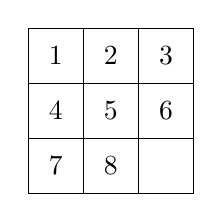
\begin{tikzpicture}[scale=.7]
\draw  (0,0) rectangle node{1} (1,-1);
\draw  (1,0) rectangle node{2} (2,-1);
\draw  (2,0) rectangle node{3} (3,-1);
\draw  (0,-1) rectangle node{4} (1,-2);
\draw  (1,-1) rectangle node{5} (2,-2);
\draw  (2,-1) rectangle node{6} (3,-2);
\draw  (0,-2) rectangle node{7} (1,-3);
\draw  (1,-2) rectangle node{8} (2,-3);
\draw  (2,-2) rectangle node{} (3,-3);
\end{tikzpicture}
\end{center}
wird dargestellt durch:
\begin{lstlisting}
[ [1,2,3], 
  [4,5,6], 
  [7,8,9] ]	% 9 steht für ein leeres Feld
\end{lstlisting}
Implementierung:
\begin{lstlisting}[language=Prolog]
% Leerstelle in Zeile verschieben
sr( [9,A,B], [A,9,B]).
sr( [A,9,B], [A,B,9]).
shiftr(X,Y) :- sr(X,Y); sr(Y,X).	% findet mögliche Zeilenverschiebungen.
 
adjr( [X,  R2, R3], [Y,  R2, R3]) :- shiftr(X, Y).	% Verschiebe 1. Zeile, wenn sie Leerstelle enthält.
adjr( [R1, X,  R3], [R1, Y,  R3]) :- shiftr(X, Y).	% Verschiebe 2.
adjr( [R1, R2,  X], [R1, R2,  Y]) :- shiftr(X, Y).	% Verschiebe 3.

% Leerstelle in Spalte verschieben (Matrix transponieren, Spalten -> Zeilen. Damit Zeilenverschiebung durchführen)
adjc( [[A1,B1,C1], [D1,E1,F1], [G1,H1,I1]], 
      [[A2,B2,C2], [D2,E2,F2], [G2,H2,I2]] ) :-
	adjr( [[A1,D1,G1], [B1,E1,H1], [C1,F1,I1]],
	      [[A2,D2,G2], [B2,E2,H2], [C2,F2,I2]] ).  
 
% Leerstelle in Zeile oder Spalte verschieben
adj(Board1, Board2) :-
	adjr(Board1, Board2);
	adjc(Board1, Board2).
	
% Zielstellung
goal( [[1,2,3],
       [4,5,6],
       [7,8,9]] ).

% Pretty-Printer
printB(Board) :- maplist(writeln, Board), write('\n').
print(Boards) :- maplist(printB, Boards).
\end{lstlisting}

\subsection{Spiele mit Gegner}

Es gibt zwei Spieler: Min, Max. Im Spielbaum stellen wir Min durch $\triangledown$, Max durch $\triangle$ dar. Im Spielbaum gibt es Endzustände und eine Nutzenfunktion, die den Nutzen eines Knotens für Max angibt.\\
Der einfachste Fall einer Nutzenfunktion ist eine Funktion mit drei Werten:
\begin{itemize}
\item[1:] Max hat gewonnen
\item[0:] unentschieden
\item[-1:] Min hat gewonnen
\end{itemize}
Max versucht die Nutzenfunktion zu maximieren, Min versucht sie zu minimieren.\\
Für Endzustände lässt nich die Nutzenfunktion leicht angeben.

\paragraph{Beispiel} Suchbaum für Tic-Tac-Toe, Max setzt $\times$, Min setzt $\circ$

\begin{center}
\begin{tikzpicture}[scale=.4]

\draw  (0,-4) rectangle (1,-3);
\draw  (1,-4) rectangle (2,-3);
\draw  (2,-4) rectangle (3,-3);
\draw  (0,-5) rectangle (1,-4);
\draw  (1,-5) rectangle (2,-4);
\draw  (2,-5) rectangle (3,-4);
\draw  (0,-6) rectangle (1,-5);
\draw  (1,-6) rectangle (2,-5);
\draw  (2,-6) rectangle (3,-5);

\draw  (-5,-9) rectangle node{$\times$}(-4,-8);
\draw  (-4,-9) rectangle (-3,-8);
\draw  (-3,-9) rectangle (-2,-8);
\draw  (-5,-10) rectangle (-4,-9);
\draw  (-4,-10) rectangle (-3,-9);
\draw  (-3,-10) rectangle (-2,-9);
\draw  (-5,-11) rectangle (-4,-10);
\draw  (-4,-11) rectangle (-3,-10);
\draw  (-3,-11) rectangle (-2,-10);

\draw  (5,-9) rectangle (6,-8);
\draw  (6,-9) rectangle (7,-8);
\draw  (7,-9) rectangle (8,-8);
\draw  (5,-10) rectangle (6,-9);
\draw  (6,-10) rectangle (7,-9);
\draw  (7,-10) rectangle (8,-9);
\draw  (5,-11) rectangle (6,-10);
\draw  (6,-11) rectangle (7,-10);
\draw  (7,-11) rectangle node{$\times$} (8,-10);

\draw  (-9,-14) rectangle node{$\times$} (-8,-13);
\draw  (-8,-14) rectangle node{$\circ$} (-7,-13);
\draw  (-7,-14) rectangle (-6,-13);
\draw  (-9,-15) rectangle (-8,-14);
\draw  (-8,-15) rectangle (-7,-14);
\draw  (-7,-15) rectangle (-6,-14);
\draw  (-9,-16) rectangle (-8,-15);
\draw  (-8,-16) rectangle (-7,-15);
\draw  (-7,-16) rectangle (-6,-15);

\draw  (-1,-14) rectangle node{$\times$} (0,-13);
\draw  (0,-14) rectangle (1,-13);
\draw  (1,-14) rectangle (2,-13);
\draw  (-1,-15) rectangle (0,-14);
\draw  (0,-15) rectangle (1,-14);
\draw  (1,-15) rectangle (2,-14);
\draw  (-1,-16) rectangle (0,-15);
\draw  (0,-16) rectangle (1,-15);
\draw  (1,-16) rectangle node{$\circ$} (2,-15);
\node at (-4,-14) {…};
\node at (1,-9) {…};
\draw (0.5,-6) -- (-3.5,-8);
\draw (1.5,-6) -- (0,-7.5);
\draw (2.5,-6) -- (6.5,-8);
\draw (-4.5,-11) -- (-7.5,-13);
\draw (-3.5,-11) -- (-4,-13);

\draw (-2.5,-11) -- (0.5,-13);
\draw (-7.5,-16) -- (-9.5,-19) node[below]{…};
\draw (0.5,-16) -- (2,-19) node[below]{…};
\draw (6.5,-11) -- (7.5,-14) node[below]{…};
\end{tikzpicture}
\end{center}

\begin{center}
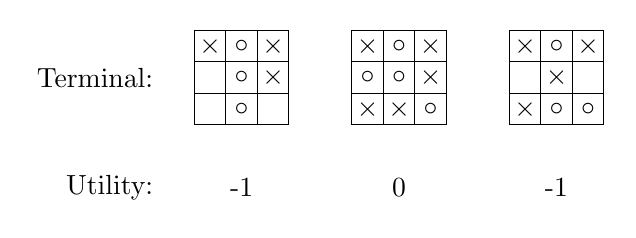
\begin{tikzpicture}[scale=.4]
\draw  (-5,-4) rectangle node{$\times$} (-4,-3);
\draw  (-4,-4) rectangle node{$\circ$} (-3,-3);
\draw  (-3,-4) rectangle node{$\times$} (-2,-3);
\draw  (-5,-5) rectangle (-4,-4);
\draw  (-4,-5) rectangle node{$\circ$} (-3,-4);
\draw  (-3,-5) rectangle node{$\times$} (-2,-4);
\draw  (-5,-6) rectangle (-4,-5);
\draw  (-4,-6) rectangle node{$\circ$} (-3,-5);
\draw  (-3,-6) rectangle (-2,-5);

\draw  (0,-4) rectangle node{$\times$} (1,-3);
\draw  (1,-4) rectangle node{$\circ$} (2,-3);
\draw  (2,-4) rectangle node{$\times$} (3,-3);
\draw  (0,-5) rectangle node{$\circ$} (1,-4);
\draw  (1,-5) rectangle node{$\circ$} (2,-4);
\draw  (2,-5) rectangle node{$\times$} (3,-4);
\draw  (0,-6) rectangle node{$\times$} (1,-5);
\draw  (1,-6) rectangle node{$\times$} (2,-5);
\draw  (2,-6) rectangle node{$\circ$} (3,-5);

\draw  (5,-4) rectangle node{$\times$} (6,-3);
\draw  (6,-4) rectangle node{$\circ$} (7,-3);
\draw  (7,-4) rectangle node{$\times$} (8,-3);
\draw  (5,-5) rectangle (6,-4);
\draw  (6,-5) rectangle node{$\times$} (7,-4);
\draw  (7,-5) rectangle (8,-4);
\draw  (5,-6) rectangle node{$\times$} (6,-5);
\draw  (6,-6) rectangle node{$\circ$} (7,-5);
\draw  (7,-6) rectangle node{$\circ$} (8,-5);
\node at (-3.5,-8) {-1};
\node at (1.5,-8) {0};
\node at (6.5,-8) {-1};
\node at (-6,-4.5) [left] {Terminal:};
\node at (-6,-8) [left] {Utility:};
\end{tikzpicture}
\end{center}

\subsubsection{Minimax}
Da wir nicht wissen, wie der Gegner zieht, betrachten wir alle möglichen Züge des Gegners und nehmen an, dass dieser optimal spielt. Damit berechnen wir einen Nutzenwert für jeden Knoten (minmax-Wert). Dieser ergibt sich als:
\begin{itemize}
\item Maximum der Bewertungen der Nachfolgeknoten, wenn Max am Zug ist,
\item Minimum der Bewertungen der Nachfolgeknoten, wenn Min am Zug ist.
\end{itemize}
Damit erhalten wir:
$$ \mathrm{minimax}(n) =\begin{cases}
\mathrm{utility}(n) & \text{, wenn }n \text{ ein Endzustand ist}\\
\max\{ \mathrm{minimax}(s)\;|\; s \text{ ist Nachfolger von }n\} & \text{, wenn }n \text{ ein Max-Knoten ist}\\
\min\{ \mathrm{minimax}(s)\;|\; s \text{ ist Nachfolger von }n\} & \text{, wenn }n \text{ ein Min-Knoten ist}\\
\end{cases} $$
\begin{center}
\begin{tikzpicture}[scale=.5]
\node (v2) at (0,0) {$\triangle$ 1};
\node (v1) at (-3,-3) {1};
\node (v4) at (0,-3) {0};
\node (v3) at (3,-3) {-1};
\draw (v1) -- (v2) -- (v3);
\draw (v2) -- (v4);
\end{tikzpicture} \quad
\begin{tikzpicture}[scale=.5]
\node (v2) at (0,0) {$\triangledown$ -1};
\node (v1) at (-3,-3) {1};
\node (v4) at (0,-3) {0};
\node (v3) at (3,-3) {-1};
\draw (v1) -- (v2) -- (v3);
\draw (v2) -- (v4);
\end{tikzpicture}
\end{center}

\paragraph{Beispiel}
\begin{center}
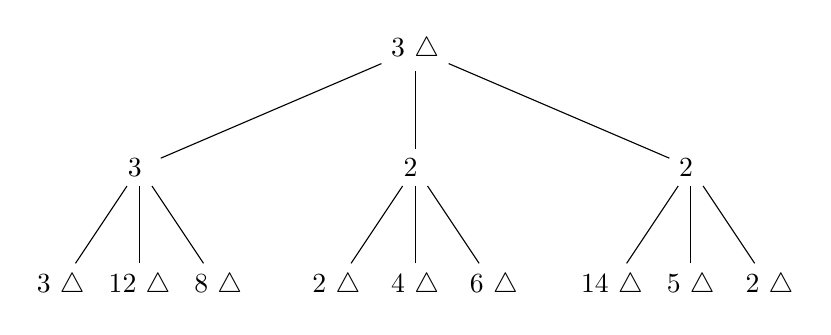
\begin{tikzpicture}[scale=.5]
\node (v2) at (0,0) {3 $\triangle$};
\node (v1) at (-7,-3) {3 $\triangledown$};
\node (v4) at (0,-3) {2 $\triangledown$};
\node (v3) at (7,-3) {2 $\triangledown$};
\draw (v1) -- (v2) -- (v3);
\draw (v2) -- (v4);
\node (v5) at (-9,-6) {3 $\triangle$};
\node (v7) at (-7,-6) {12 $\triangle$};
\node (v6) at (-5,-6) {8 $\triangle$};
\node (v8) at (-2,-6) {2 $\triangle$};
\node (v10) at (0,-6) {4 $\triangle$};
\node (v9) at (2,-6) {6 $\triangle$};
\node (v11) at (5,-6) {14 $\triangle$};
\node (v13) at (7,-6) {5 $\triangle$};
\node (v12) at (9,-6) {2 $\triangle$};
\draw (v5) -- (v1) -- (v6);
\draw (v1) -- (v7);
\draw (v8) -- (v4) -- (v9);
\draw (v10) -- (v4);
\draw (v11) -- (v3) -- (v12);
\draw (v13) -- (v3);
\end{tikzpicture}
\end{center}\bigskip
Laufzeit der Minimax-Berechnung: $O(b^d)$ für Spielbaum mit (konstanten) Verzweigungsfaktor $b$ und Tiefe $d$.\\
Um die Laufzeit zu verkürzen rechnen wir Minimax-Werte nur für solche Knoten, die das Ergebnis verändern können.
\paragraph{Beispiel}
\begin{center}
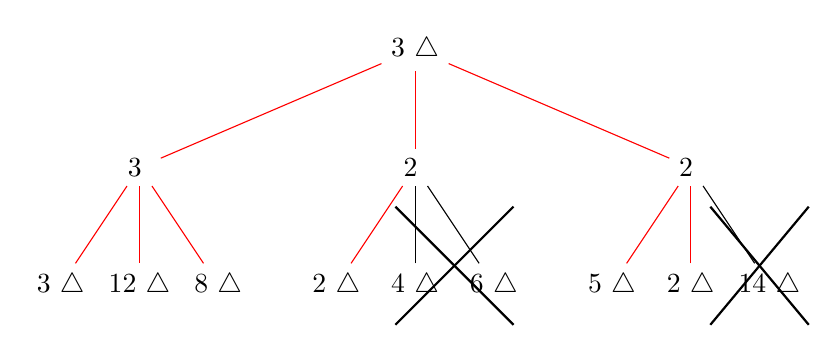
\begin{tikzpicture}[scale=.5]
\node (v2) at (0,0) {3 $\triangle$};
\node (v1) at (-7,-3) {3 $\triangledown$};
\node (v4) at (0,-3) {2 $\triangledown$};
\node (v3) at (7,-3) {2 $\triangledown$};
\draw [red] (v1) -- (v2) -- (v3);
\draw [red] (v2) -- (v4);
\node (v5) at (-9,-6) {3 $\triangle$};
\node (v7) at (-7,-6) {12 $\triangle$};
\node (v6) at (-5,-6) {8 $\triangle$};
\node (v8) at (-2,-6) {2 $\triangle$};
\node (v10) at (0,-6) {4 $\triangle$};
\node (v9) at (2,-6) {6 $\triangle$};
\node (v11) at (5,-6) {5 $\triangle$};
\node (v13) at (7,-6) {2 $\triangle$};
\node (v12) at (9,-6) {14 $\triangle$};
\draw [red] (v5) -- (v1) -- (v6);
\draw [red] (v1) -- (v7);
\draw [red] (v8) -- (v4);
\draw (v4) -- (v9);
\draw (v10) -- (v4);
\draw [red] (v11) -- (v3);
\draw (v3) -- (v12);
\draw [red](v13) -- (v3);
\draw [thick](-0.5,-7) -- (2.5,-4);
\draw [thick](-0.5,-4) -- (2.5,-7);
\draw [thick](7.5,-7) -- (10,-4);
\draw [thick](7.5,-4) -- (10,-7);
\end{tikzpicture}
\end{center}
Die Tiefensuche kann im zweiten Zweig abgebrochen werden, da bereits ein (potentielles) Minimum für den minmax-Wert gefunden wurde. Dies ist schon geringer, als das Minimum vom ersten Zweig. Damit braucht der nicht rot markierte Pfad zu Knoten 4 und 6 nicht mehr betrachtet werden. Gleiches gilt für den Pfad zum Koten 14 im dritten Zweig.

\subsubsection{Alpha-Beta-Algorithmus}
Der $\alpha$-$\beta$-Algorithmus schneidet Zweige des Suchbaums ab, wenn die Werte der darin enthaltenen Knoten den Minimax-Wert des aktuellen Knotens nicht verändern.\\
Dann wird während der Suche für jeden Knoten ein Intervall $[\alpha, \beta]$ mitgeführt, das angibt, in welchem Bereich sich der Minimax-Wert befindet.

Regeln für das Beschneiden des Suchbaums (Pruning):
\begin{itemize}
\item Ist der $\beta$-Wert eines Min-Knotens $\leq$ $\alpha$-Wert des Vater-Max-Kontens, so wird der Min-Knoten nicht weiter untersucht.
\begin{center}
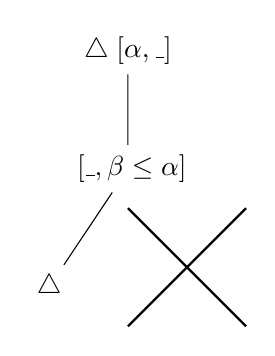
\begin{tikzpicture}[scale=.5]
\node (v3) at (0,0) {$\triangle\; [\alpha, \_]$};
\node (v2) at (0,-3) {$\triangledown\; [\_, \beta \leq \alpha]$};
\node (v1) at (-2,-6) {$\triangle$};
\draw (v1) -- (v2) -- (v3);
\draw [thick] (0,-4) -- (3,-7);
\draw [thick] (0,-7) -- (3,-4);
\end{tikzpicture}
\end{center}
\item Ist der $\alpha$-Wert eines Max-Knotens $\geq$ $\beta$-Wert des Vater-Min-Knotens, so wird der Max-Knoten nicht weiter untersucht.
\begin{center}
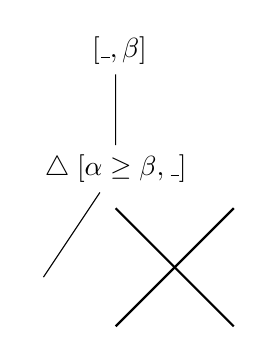
\begin{tikzpicture}[scale=.5]
\node (v3) at (0,0) {$\triangledown\; [\_,\beta]$};
\node (v2) at (0,-3) {$\triangle\; [\alpha \geq \beta, \_]$};
\node (v1) at (-2,-6) {$\triangledown$};
\draw (v1) -- (v2) -- (v3);
\draw [thick] (0,-4) -- (3,-7);
\draw [thick] (0,-7) -- (3,-4);
\end{tikzpicture}
\end{center}
\end{itemize}

\paragraph{Beispiel} Suchbaum von oben:\\
1. Schritt:
\begin{center}
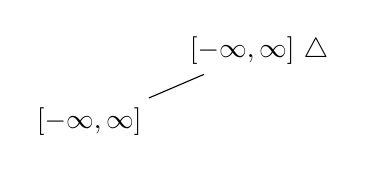
\begin{tikzpicture}[scale=.3]
\node (v2) at (0,0) {$[-\infty, \infty]$ $\triangle$};
\node (v1) at (-7,-3) {$[-\infty, \infty]$ $\triangledown$};c
\draw (v2) -- (v1);
\end{tikzpicture}
\end{center}
2. Schritt:
\begin{center}
\begin{tikzpicture}[scale=.3]
\node (v2) at (0,0) {$[-\infty, \infty]$ $\triangle$};
\node (v1) at (-7,-3) {$[-\infty, 3]$ $\triangledown$};c
\draw (v2) -- (v1);
\node (v3) at (-10,-6) {3 $\triangle$};
\draw (v3) -- (v1);
\end{tikzpicture}
\end{center}
3. Schritt:
\begin{center}
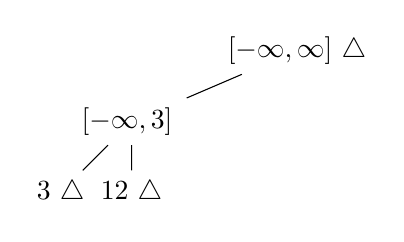
\begin{tikzpicture}[scale=.3]
\node (v2) at (0,0) {$[-\infty, \infty]$ $\triangle$};
\node (v1) at (-7,-3) {$[-\infty, 3]$ $\triangledown$};c
\draw (v2) -- (v1);
\node (v3) at (-10,-6) {3 $\triangle$};
\draw (v3) -- (v1);
\node (v4) at (-7,-6) {12 $\triangle$};
\draw (v4) -- (v1);
\end{tikzpicture}
\end{center}
4. Schritt:
\begin{center}
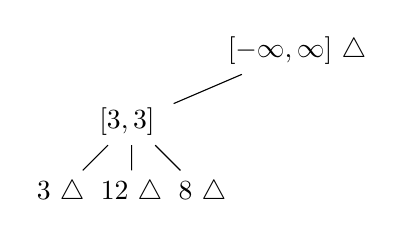
\begin{tikzpicture}[scale=.3]
\node (v2) at (0,0) {$[-\infty, \infty]$ $\triangle$};
\node (v1) at (-7,-3) {$[3, 3]$ $\triangledown$};c
\draw (v2) -- (v1);
\node (v3) at (-10,-6) {3 $\triangle$};
\draw (v3) -- (v1);
\node (v4) at (-7,-6) {12 $\triangle$};
\draw (v4) -- (v1);
\node (v5) at (-4,-6) {8 $\triangle$};
\draw (v5) -- (v1);
\end{tikzpicture}
\end{center}
5. Schritt:
\begin{center}
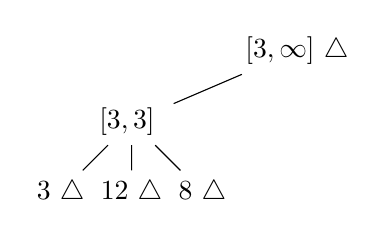
\begin{tikzpicture}[scale=.3]
\node (v2) at (0,0) {$[3, \infty]$ $\triangle$};
\node (v1) at (-7,-3) {$[3, 3]$ $\triangledown$};
\draw (v2) -- (v1);
\node (v3) at (-10,-6) {3 $\triangle$};
\draw (v3) -- (v1);
\node (v4) at (-7,-6) {12 $\triangle$};
\draw (v4) -- (v1);
\node (v5) at (-4,-6) {8 $\triangle$};
\draw (v5) -- (v1);
\end{tikzpicture}
\end{center}
6. Schritt:
\begin{center}
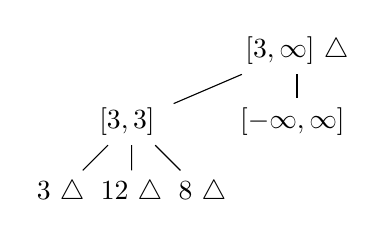
\begin{tikzpicture}[scale=.3]
\node (v2) at (0,0) {$[3, \infty]$ $\triangle$};
\node (v1) at (-7,-3) {$[3, 3]$ $\triangledown$};
\draw (v2) -- (v1);
\node (v3) at (-10,-6) {3 $\triangle$};
\draw (v3) -- (v1);
\node (v4) at (-7,-6) {12 $\triangle$};
\draw (v4) -- (v1);
\node (v5) at (-4,-6) {8 $\triangle$};
\draw (v5) -- (v1);
\node (v6) at (0,-3) {$[-\infty, \infty]$ $\triangledown$};
\draw (v2) -- (v6);
\end{tikzpicture}
\end{center}
7. Schritt:
\begin{center}
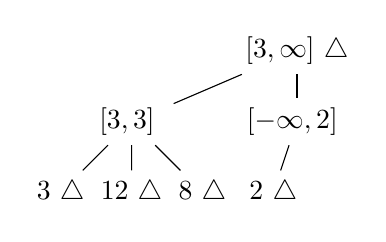
\begin{tikzpicture}[scale=.3]
\node (v2) at (0,0) {$[3, \infty]$ $\triangle$};
\node (v1) at (-7,-3) {$[3, 3]$ $\triangledown$};
\draw (v2) -- (v1);
\node (v3) at (-10,-6) {3 $\triangle$};
\draw (v3) -- (v1);
\node (v4) at (-7,-6) {12 $\triangle$};
\draw (v4) -- (v1);
\node (v5) at (-4,-6) {8 $\triangle$};
\draw (v5) -- (v1);
\node (v6) at (0,-3) {$[-\infty, 2]$ $\triangledown$};
\draw (v2) -- (v6);
\node (v7) at (-1,-6) {2 $\triangle$};
\draw (v7) -- (v6);
\end{tikzpicture}
\end{center}
8. Schritt:
\begin{center}
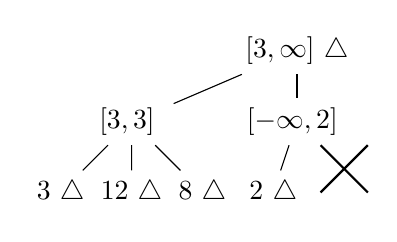
\begin{tikzpicture}[scale=.3]
\node (v2) at (0,0) {$[3, \infty]$ $\triangle$};
\node (v1) at (-7,-3) {$[3, 3]$ $\triangledown$};
\draw (v2) -- (v1);
\node (v3) at (-10,-6) {3 $\triangle$};
\draw (v3) -- (v1);
\node (v4) at (-7,-6) {12 $\triangle$};
\draw (v4) -- (v1);
\node (v5) at (-4,-6) {8 $\triangle$};
\draw (v5) -- (v1);
\node (v6) at (0,-3) {$[-\infty, 2]$ $\triangledown$};
\draw (v2) -- (v6);
\node (v7) at (-1,-6) {2 $\triangle$};
\draw (v7) -- (v6);
\draw [thick] (1,-4) -- (3,-6);
\draw [thick] (1,-6) -- (3,-4);
\end{tikzpicture}
\end{center}
Analog:
\begin{center}
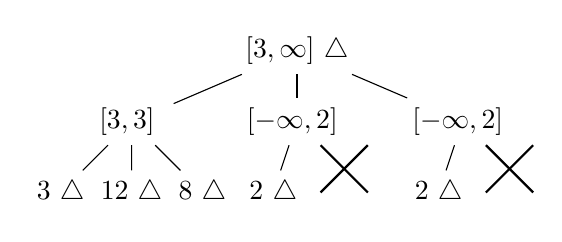
\begin{tikzpicture}[scale=.3]
\node (v2) at (0,0) {$[3, \infty]$ $\triangle$};
\node (v1) at (-7,-3) {$[3, 3]$ $\triangledown$};
\draw (v2) -- (v1);
\node (v3) at (-10,-6) {3 $\triangle$};
\draw (v3) -- (v1);
\node (v4) at (-7,-6) {12 $\triangle$};
\draw (v4) -- (v1);
\node (v5) at (-4,-6) {8 $\triangle$};
\draw (v5) -- (v1);
\node (v6) at (0,-3) {$[-\infty, 2]$ $\triangledown$};
\draw (v2) -- (v6);
\node (v7) at (-1,-6) {2 $\triangle$};
\draw (v7) -- (v6);
\draw [thick] (1,-4) -- (3,-6);
\draw [thick] (1,-6) -- (3,-4);
\node (v6) at (7,-3) {$[-\infty, 2]$ $\triangledown$};
\draw (v2) -- (v6);
\node (v7) at (6,-6) {2 $\triangle$};
\draw (v7) -- (v6);
\draw [thick] (8,-4) -- (10,-6);
\draw [thick] (8,-6) -- (10,-4);
\end{tikzpicture}
\end{center}
Und damit letztendlich:
\begin{center}
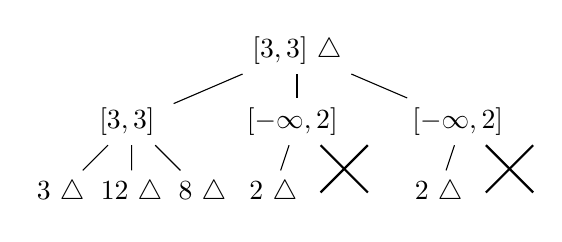
\begin{tikzpicture}[scale=.3]
\node (v2) at (0,0) {$[3, 3]$ $\triangle$};
\node (v1) at (-7,-3) {$[3, 3]$ $\triangledown$};
\draw (v2) -- (v1);
\node (v3) at (-10,-6) {3 $\triangle$};
\draw (v3) -- (v1);
\node (v4) at (-7,-6) {12 $\triangle$};
\draw (v4) -- (v1);
\node (v5) at (-4,-6) {8 $\triangle$};
\draw (v5) -- (v1);
\node (v6) at (0,-3) {$[-\infty, 2]$ $\triangledown$};
\draw (v2) -- (v6);
\node (v7) at (-1,-6) {2 $\triangle$};
\draw (v7) -- (v6);
\draw [thick] (1,-4) -- (3,-6);
\draw [thick] (1,-6) -- (3,-4);
\node (v6) at (7,-3) {$[-\infty, 2]$ $\triangledown$};
\draw (v2) -- (v6);
\node (v7) at (6,-6) {2 $\triangle$};
\draw (v7) -- (v6);
\draw [thick] (8,-4) -- (10,-6);
\draw [thick] (8,-6) -- (10,-4);
\end{tikzpicture}
\end{center}














